\chapter{Introduction}
\label{chp:introduction}
\Acp{cnn} are great \cite{goodfellow_deep_2016} because a \ac{cnn} is good at classifying images.

% An empty line between text starts a new paragraph
A depiction of the gripper of the \ac{cob4} used at \ac{ipa} is given in Figure~\ref{fig:Grippers}. % References (figures, tables, equations, algorithms, chapters, etc... ) always with capital letter.

\par\bigskip  % some further space, can also be used between subfigures for more vertical space
%\par\medskip
%\par\smallskip

\begin{figure}[htbp]
	\centering
	\begin{subfigure}{0.49\textwidth}
		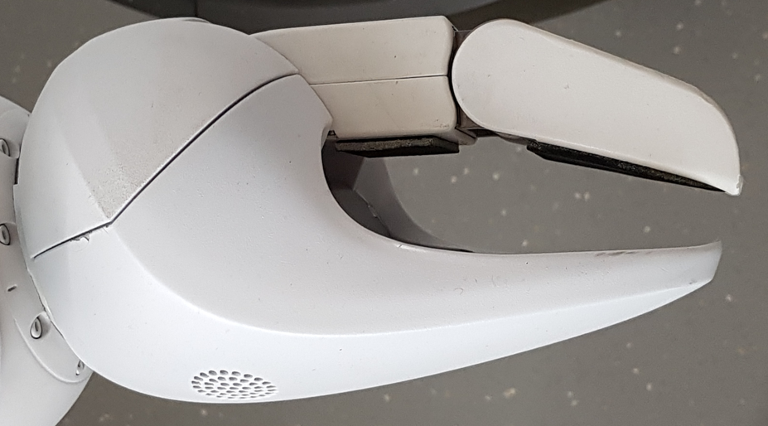
\includegraphics[height=0.15\textheight, center]{resources/figures/introduction/cob4_gripper}
		\caption{Real-World}
	\end{subfigure}
	\begin{subfigure}{0.49\textwidth}
		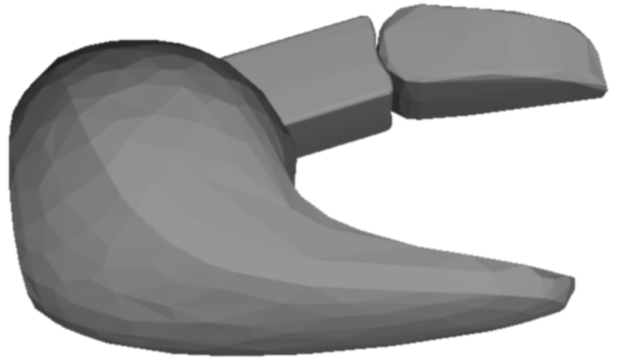
\includegraphics[height=0.15\textheight, center]{resources/figures/introduction/cob4_gripper_sim}
		\caption{Simulation}
	\end{subfigure}
	\caption[Two-finger gripper of the \acs{cob4}]{Two-finger gripper of the \acs{cob4} used at \acs{ipa}}  % caption below images
	\label{fig:Grippers}
\end{figure}
% Use always the short (e.g. acs) version for acronyms in captions to avoid having the full string printed in the list of figures. Take a look at the documentation of the acro package for further information.

\noindent Some hyperparameters are explained in Table~\ref{tab:hyperparameters} below.  % \noindent suppresses the paragraph indentation

% Nice tables only have horizontal lines. Avoid vertical lines for a better appearance.
\begingroup
\renewcommand\arraystretch{1.3}  % more space between rows (also affects equations, therefore use a local group)
\begin{table}[b!]  % force on bottom
\centering
\caption{Hyperparameters}  % caption above tables
\label{tab:hyperparameters}
\begin{tabularx}{\linewidth}{lX}
	\toprule
	\textbf{Parameter} & \textbf{Description}\\
	\midrule
Learning Rate & This is the most important hyperparameter to tune. It defines the stepsize to take in negative gradient direction to reduce the overall error of the neural network.\\
Batch Size & This specifies the amount of samples processed in one update of the neural network.\\
	\bottomrule
\end{tabularx}
\end{table}
\endgroup

